\newpage
\section{Ôn tập chương 5}

\def\thoigian{90}%--Thời gian
\de{Đề số 1}{Chương V. Phương trình mặt phẳng, đường thẳng, mặt cầu}

\begin{center}
	\textbf{PHẦN 1 - CÂU TRẮC NGHIỆM BỐN PHƯƠNG ÁN}
\end{center}
\Opensolutionfile{ans}[ans/ans-TN-ONTAPCHUONG-DE1]

%Câu 1
\begin{ex}%[Dự án D - Đề cương 3 khối 10-11-12 NH25-26 - Nguyễn Tiến]
	Trong không gian với hệ toạ độ $Oxyz$, cho mặt phẳng $(P)\colon 2x-y+4z-5=0$. Vectơ nào sau đây là một vectơ pháp tuyến của mặt phẳng $(P)$?
	\choice
	{\True $\overrightarrow{n}_1=(2;-1;4)$}
	{$\overrightarrow{n}_2=(2;1;4)$}
	{$\overrightarrow{n}_3=(2;-1;-4)$}
	{$\overrightarrow{n}_4=(1;-1;4)$}
	\loigiai{
		Từ các phương án, ta thấy một vectơ pháp tuyến của mặt phẳng $(P)$ là $\overrightarrow{n}_1=(2;-1;4)$.
	}
\end{ex}
%Câu 2
\begin{ex}%[Dự án D - Đề cương 3 khối 10-11-12 NH25-26 - Nguyễn Tiến]
	[\textit{Trích đề thi thử Sở Ninh Bình, lần 2 - Năm học 2024-2025}]
	Trong không gian với hệ toạ độ $Oxyz$, khoảng cách từ điểm $A(3;-2;4)$ đến mặt phẳng $(Oxz)$ bằng
	\choice
	{$4$}
	{$5$}
	{$3$}
	{\True $2$}
	\loigiai{
		Mặt phẳng $(Oxz)$ có phương trình là $y=0$.\\
		Khi đó $\mathrm{d}(A,(Oxz))=\left|-2\right|=2$.
	}
\end{ex}
%Câu 3
\begin{ex}%[Dự án D - Đề cương 3 khối 10-11-12 NH25-26 - Nguyễn Tiến]
	[\textit{Trích đề thi thử Trường THPT Văn Quán, Vĩnh Phúc - Năm học 2024-2025}]
	Trong không gian với hệ toạ độ $Oxyz$, đường thẳng $d\colon \heva{& x=-1+2t\\& y=2-t\\& z=3t}$ có một vectơ chỉ phương là
	\choice
	{$\overrightarrow{u}_1=(2;1;3)$}
	{$\overrightarrow{u}_2=(-1;2;0)$}
	{\True $\overrightarrow{u}_4=(2;-1;3)$}
	{$\overrightarrow{u}_3=(-1;2;3)$}
	\loigiai{
		Đường thẳng $d$ có một vectơ chỉ phương là $\overrightarrow{u}_4=(2;-1;3)$.
	}
\end{ex}
%Câu 4
\begin{ex}%[Dự án D - Đề cương 3 khối 10-11-12 NH25-26 - Nguyễn Tiến]
	[\textit{Trích đề thi thử Trường THCS-THPT Nguyễn Khuyến - Lê Thánh Tông, TPHCM - Năm học 2024-2025}]
	Trong không gian với hệ toạ độ $Oxyz$, đường thẳng $Oy$ có phương trình tham số là
	\choice
	{$\heva{& x=t\\& y=t\\& z=t}$}
	{\True $\heva{& x=0\\& y=2+t\\& z=0}$}
	{$\heva{& x=0\\& y=0\\& z=t}$}
	{$\heva{& x=t\\& y=0\\& z=0}$}
	\loigiai{
		Ta có $Oy$ đi qua điểm $M(0;2;0)$ và có vectơ chỉ phương $\overrightarrow{j}=(0;1;0)$.\\
		Suy ra $Oy$ có phương trình tham số là $\heva{& x=0\\& y=2+t\\& z=0}$ (với $t\in \mathbb{R}$).
	}
\end{ex}
%Câu 5
\begin{ex}%[Dự án D - Đề cương 3 khối 10-11-12 NH25-26 - Nguyễn Tiến]
	Trong không gian với hệ toạ độ $Oxyz$, cho mặt cầu $(S)\colon x^2+(y-4)^2+(z-1)^2=25$. Toạ độ tâm $I$ và bán kính $R$ của mặt cầu $(S)$ là
	\choice
	{$I(0;-4;-1)$, $R=25$}
	{$I(0;-4;-1)$, $R=5$}
	{$I(0;4;1)$, $R=25$}
	{\True $I(0;4;1)$, $R=5$}
	\loigiai{
		Mặt cầu $(S)$ có tâm $I(0;4;1)$ và bán kính $R=5$.
	}
\end{ex}
%Câu 6
\begin{ex}%[Dự án D - Đề cương 3 khối 10-11-12 NH25-26 - Nguyễn Tiến]
	Trong không gian với hệ toạ độ $Oxyz$, phương trình của mặt cầu tâm $I(2;1;-3)$ và có đường kính bằng $18$ là
	\choice
	{\True $(x-2)^2+(y-1)^2+(z+3)^2=81$}
	{$(x+2)^2+(y+1)^2+(z-3)^2=81$}
	{$(x-2)^2+(y-1)^2+(z+3)^2=9$}
	{$(x+2)^2+(y+1)^2+(z-3)^2=9$}
	\loigiai{
		Phương trình mặt cầu có tâm $I(2;1;-3)$ và bán kính $R=\dfrac{18}{2}=9$ là
		$$(x-2)^2+(y-1)^2+(z+3)^2=81.$$
	}
\end{ex}
%Câu 7
\begin{ex}%[Dự án D - Đề cương 3 khối 10-11-12 NH25-26 - Nguyễn Tiến]
	Trong không gian với hệ toạ độ $Oxyz$, cho điểm $A(0;-3;2)$ và mặt phẳng $(P)\colon 2x-y+3z+5=0$. Mặt phẳng $(Q)$ đi qua $A$ và song song với $(P)$ có phương trình là
	\choice
	{$2x-y+3z+9=0$}
	{$2x+y+3z-3=0$}
	{$2x+y+3z+3=0$}
	{\True $2x-y+3z-9=0$}
	\loigiai{
		Mặt phẳng $(Q)$ song song với $(P)$ có phương trình dạng
		$$2x-y+3z+d=0 \text{ (với } d\neq 5).$$
		Lại có $A\in (Q)$ nên suy ra $2\cdot 0-(-3)+3\cdot 2+d=0 \Leftrightarrow d=-9$ (nhận).\\
		Vậy $(Q)\colon 2x-y+3z-9=0$.
	}
\end{ex}
%Câu 8
\begin{ex}%[Dự án D - Đề cương 3 khối 10-11-12 NH25-26 - Nguyễn Tiến]
	Trong không gian với hệ toạ độ $Oxyz$, cho hai điểm $A(2;3;-1)$, $B(-1;0;1)$. Mặt phẳng trung trực của đoạn $AB$ có phương trình là
	\choice
	{$3x+3y-2z+6=0$}
	{\True $3x+3y-2z-6=0$}
	{$3x+3y+2z-6=0$}
	{$3x-3y-2z-6=0$}
	\loigiai{
		Ta có $\overrightarrow{AB}=(3;3;-2)$ và $I\left(\dfrac{1}{2};\dfrac{3}{2};0\right)$ là trung điểm của đoạn $AB$.\\
		Vậy mặt phẳng trung trực của đoạn $AB$ có phương trình là
		$$3\cdot \left(x-\dfrac{1}{2}\right)+3\cdot \left(y-\dfrac{3}{2}\right)-2z=0 \Leftrightarrow 3x+3y-2z-6=0.$$
	}
\end{ex}
%Câu 9
\begin{ex}%[Dự án D - Đề cương 3 khối 10-11-12 NH25-26 - Nguyễn Tiến]
	[\textit{Trích đề thi thử Trường THPT Chuyên Vĩnh Phúc, Vĩnh Phúc - Năm học 2024-2025}]
	Trong không gian với hệ toạ độ $Oxyz$, cho hai điểm $M(-1;-1;2)$ và $N(1;3;4)$. Đường thẳng $MN$ có phương trình chính tắc là
	\choice
	{$\dfrac{x-1}{2}=\dfrac{y-1}{4}=\dfrac{z+2}{2}$}
	{\True $\dfrac{x+1}{1}=\dfrac{y+1}{2}=\dfrac{z-2}{1}$}
	{$\dfrac{x-1}{2}=\dfrac{y-1}{2}=\dfrac{z+2}{1}$}
	{$\dfrac{x+1}{2}=\dfrac{y+3}{4}=\dfrac{z+4}{2}$}
	\loigiai{
		Ta có $\overrightarrow{MN}=(2;4;2)=2\cdot (1;2;1)$.\\
		Đường thẳng $MN$ đi qua điểm $M(-1;-1;2)$ và nhận $\overrightarrow{u}=(1;2;1)$ làm vectơ chỉ phương.\\
		Vậy đường thẳng $MN$ có phương trình chính tắc là $\dfrac{x+1}{1}=\dfrac{y+1}{2}=\dfrac{z-2}{1}$.
	}
\end{ex}
%Câu 10
\begin{ex}%[Dự án D - Đề cương 3 khối 10-11-12 NH25-26 - Nguyễn Tiến]
	[\textit{Trích đề thi thử Trường THCS-THPT Bình Sơn, Vĩnh Phúc - Năm học 2024-2025}]
	Trong không gian với hệ toạ độ $Oxyz$, cho ba điểm $A(-1;2;1)$, $B(2;-1;3)$ và $C(-2;1;2)$. Đường thẳng đi qua $A$ đồng thời vuông góc với $BC$ và trục $Oy$ có phương trình là
	\choice
	{$\heva{& x=-1+t\\& y=2\\& z=1+4t}$}
	{\True $\heva{& x=-1-t\\& y=2\\& z=1+4t}$}
	{$\heva{& x=-1-t\\& y=0\\& z=1-4t}$}
	{$\heva{& x=-1+t\\& y=2t\\& z=1+4t}$}
	\loigiai{
		Ta có $\overrightarrow{CB}=(4;-2;1)$ và $\overrightarrow{j}=(0;1;0)$.\\
		Suy ra $\left[\overrightarrow{CB},\overrightarrow{j}\right]=(-1;0;4)$.\\
		Đường thẳng đi qua $A$ đồng thời vuông góc với $BC$ và trục $Oy$ có một vectơ chỉ phương $\overrightarrow{u}=(-1;0;4)$.\\
		Suy ra phương trình đường thẳng cần tìm là $\heva{& x=-1-t\\& y=2\\& z=1+4t.}$
	}
\end{ex}
%Câu 11
\begin{ex}%[Dự án D - Đề cương 3 khối 10-11-12 NH25-26 - Nguyễn Tiến]
	[\textit{Trích đề thi thử Trường THPT Hai Bà Trưng, Vĩnh Phúc - Năm học 2024-2025}]
	Trong không gian với hệ toạ độ $Oxyz$, trong các mặt cầu dưới đây, mặt cầu nào có bán kính $R=2$?
	\choice
	{$(S_1)\colon x^2+y^2+z^2-4x+2y+2z-3=0$}
	{$(S_2)\colon x^2+y^2+z^2-4x+2y+2z-10=0$}
	{\True $(S_3)\colon x^2+y^2+z^2-4x+2y+2z+2=0$}
	{$(S_4)\colon x^2+y^2+z^2-4x+2y+2z+5=0$}
	\loigiai{
		Xét mặt cầu $(S_3)\colon x^2+y^2+z^2-4x+2y+2z+2=0$, ta có
		$$\heva{& -2a=-4\\& -2b=2\\& -2c=2\\& d=2} \Leftrightarrow \heva{& a=2\\& b=-1\\& c=-1\\& d=2.}$$
		Suy ra bán kính $R=\sqrt{a^2+b^2+c^2-d}=\sqrt{4}=2$.
	}
\end{ex}
%Câu 12
\begin{ex}%[Dự án D - Đề cương 3 khối 10-11-12 NH25-26 - Nguyễn Tiến]
	[\textit{Trích đề thi thử Trường THPT Bình Sơn, Vĩnh Phúc - Năm học 2024-2025}]
	Trong không gian với hệ toạ độ $Oxyz$, cho điểm $I(1;4;0)$. Mặt cầu $(S)$ tâm $I$ và đi qua điểm $M(1;4;-2)$ có phương trình là
	\choice
	{\True $(x-1)^2+(y-4)^2+z^2=4$}
	{$(x-1)^2+(y-4)^2+z^2=2$}
	{$(x+1)^2+(y+4)^2+z^2=4$}
	{$(x+1)^2+(y+4)^2+z^2=2$}
	\loigiai{
		Mặt cầu $(S)$ có tâm $I$ và bán kính $R=IM=2$ có phương trình là $(x-1)^2+(y-4)^2+z^2=4$.
	}
\end{ex}

\Closesolutionfile{ans}
%\begin{center}
%	\textbf{ĐÁP ÁN}
%	\inputansbox{10}{ans/ans}	
%\end{center}



\begin{center}
	\textbf{PHẦN 2 - CÂU TRẮC NGHIỆM ĐÚNG SAI}
\end{center}
\setcounter{ex}{0}
\Opensolutionfile{ans}[ans/answer-DS-ONTAPCHUONG-DE1]

%Câu 1
\begin{ex}%[Dự án D - Đề cương 3 khối 10-11-12 NH25-26 - Nguyễn Tiến]
	[\textit{Trích đề thi thử Trường THPT Sáng Sơn, Vĩnh Phúc - Năm học 2024-2025}]
	Trong không gian với hệ toạ độ $Oxyz$, cho đường thẳng $\Delta\colon \heva{& x=1\\& y=2-3t\\& z=3+4t} (t\in \mathbb{R})$ và mặt phẳng $(P)\colon x+3y-2z+16=0$.
	\choiceTF
	{Vectơ chỉ phương của đường thẳng $\Delta$ là $\overrightarrow{a}=(1;-3;4)$}
	{\True Đường thẳng $d_1$ vuông góc với $(P)$ có vectơ chỉ phương là $\overrightarrow{u}=(1;3;-2)$}
	{Đường thẳng $\Delta$ cắt mặt phẳng $(P)$ tại điểm có tung độ bằng $2$}
	{Đường thẳng $d_2$ qua $A(1;-1;2)$, cắt và vuông góc với trục $Oz$ có vectơ chỉ phương là $\overrightarrow{u}_2=(-1;-1;0)$}
	\loigiai{
		\begin{itemchoice}
			\itemch Ta có vectơ chỉ phương của đường thẳng $\Delta$ là $\overrightarrow{a}=(0;-3;4)$.
			\itemch Ta có mặt phẳng $(P)$ có một vectơ pháp tuyến là $\overrightarrow{u}=(1;3;-2)$.\\
				Khi đó đường thẳng $d_1$ vuông góc với $(P)$ nên có một vectơ chỉ phương là $\overrightarrow{u}=(1;3;-2)$.
			\itemch Gọi $M(1; 2-3t; 3+4t)\in d$ là giao điểm cần tìm.\\
				Do $M\in (P)$ nên suy ra $1+3\cdot (2-3t)-2\cdot (3+4t)+16=0 \Leftrightarrow t=1$.\\
				Vậy đường thẳng $\Delta$ cắt mặt phẳng $(P)$ tại điểm $M(1;-1;7)$.
			\itemch Gọi $H=d_2\cap Oz$.\\
				Ta có $\heva{& d_2\perp Oz\\& A\in d_2.}$\\
				Suy ra $H$ là hình chiếu của $A$ lên $Oz$ $\Rightarrow H(0;0;2)$.\\
				Vậy đường thẳng $d_2$ có một vectơ chỉ phương là $\overrightarrow{AH}=(-1;-1;0)$.
		\end{itemchoice}
	}
\end{ex}
%Câu 2
\begin{ex}%[]%[Dự án D - Đề cương 3 khối 10-11-12 NH25-26 - Nguyễn Tiến]
	Các thiên thạch có đường kính lớn hơn $140$ m và có thể lại gần Trái Đất ở khoảng cách nhỏ hơn $7\,500\,000$ km được coi là những vật thể có khả năng va chạm gây nguy hiểm cho Trái Đất. Để theo dõi những thiên thạch này, người ta đã thiết lập các trạm quan sát các vật thể bay gần Trái Đất.\\
	Giả sử có một hệ thống quan sát có khả năng theo dõi các vật thể ở độ cao không vượt quá $6\,630$ km so với mực nước biển. Coi Trái Đất là khối cầu có bán kính $6\,370$ km. Chọn hệ trục tọa độ $Oxyz$ trong không gian có gốc $O$ tại tâm Trái Đất và đơn vị độ dài trên mỗi trục tọa độ là $1\,000$ km. Một thiên thạch (coi như một hạt) chuyển động với tốc độ không đổi theo một đường thẳng từ điểm $M(6;15;-2)$ sau một thời gian vị trí đầu tiên thiên thạch di chuyển vào phạm vi theo dõi của hệ thống quan sát là điểm $A(5;12;0)$.
	\begin{center}
		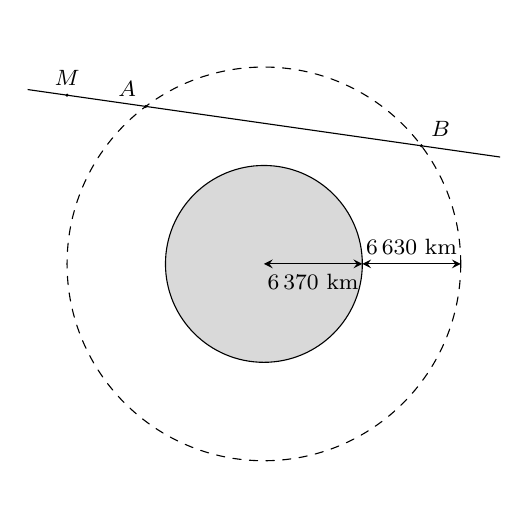
\begin{tikzpicture}[scale=0.5, font=\footnotesize, line join=round, line cap=round, >=stealth]
			\clip (-6,-6) rectangle (6,6);
			\draw[fill=gray!30] (0,0) circle(2.5cm);
			\draw[dashed] (0,0) circle(5cm);
			\draw[<->] (0,0)--(2.5,0); \node at (1.25,0) [below]{$6\,370$ km};
			\draw[<->] (2.5,0)--(5,0); \node at (3.75,0) [above]{$6\,630$ km};
			\draw[smooth,samples=300,domain=-6:6] plot(\x,{(25-(\x))/7});
			\fill (-5,4.2858) circle (1.2pt) node [above]{$M$};
			\fill (-3,4) circle (1.2pt) node [above left]{$A$};
			\fill (4,3) circle (1.2pt) node [above right]{$B$};
		\end{tikzpicture}
	\end{center}
	\choiceTF
	{\True Đường thẳng $AM$ có phương trình chính tắc là $\dfrac{x-5}{1}=\dfrac{y-12}{13}=\dfrac{z}{-2}$}
	{Trên hệ tọa độ đã cho, thiên thạch di chuyển qua điểm $N(7;18;-5)$}
	{\True Vị trí cuối cùng mà thiên thạch di chuyển trong phạm vi theo dõi của hệ thống quan sát là $B\left(-\dfrac{6}{7};-\dfrac{39}{7};\dfrac{82}{7}\right)$}
	{\True Khoảng cách giữa vị trí đầu tiên và vị trí cuối cùng mà thiên thạch di chuyển trong phạm vi theo dõi của hệ thống quan sát là $21\,915$ km (kết quả làm tròn đến hàng đơn vị theo đơn vị ki-lô-mét)}
	\loigiai{
		\begin{itemchoice}
			\itemch Đường thẳng $AM$ đi qua $A(5;12;0)$ và nhận $\overrightarrow{AM}=(1;3;-2)$ là vectơ chỉ phương.\\
				Suy ra phương trình đường thẳng $AM$ là $\dfrac{x-5}{1}=\dfrac{y-12}{13}=\dfrac{z}{-2}$.
			\itemch Ta thay toạ độ $N(7;18;-5)$ vào phương trình đường thẳng $(AM)$ ta được
				$$\dfrac{7-5}{1}=\dfrac{18-12}{3}=\dfrac{-5}{-2} \Leftrightarrow 2=2=\dfrac{5}{2} \text{ (vô lý)}.$$
				Do đó $N\notin AM$, hay thiên thạch không di chuyển qua điểm $N(7;18;-5)$.
			\itemch Ta có $B(5+t; 12+3t; -2t)\in AM$.\\
				Ngoài thực tế khoảng cách từ tâm trái đất đến vị trí cuối cùng mà thiên thạch di chuyển trong phạm vi theo dõi của hệ thống quan sát là $6\,370+6\,630=13\,000$ (km) ứng với $13$ đơn vị trên hệ trục tọa độ. Suy ra
				\allowdisplaybreaks
				\begin{eqnarray*}
					& & OB=13 \Leftrightarrow OB^2=169\\
					&\Leftrightarrow & (5+t)^2+(12+3t)^2+(-2t)^2=169\\
					&\Leftrightarrow & 14t^2+82t=0 \Leftrightarrow \hoac{& t=0\\& t=-\dfrac{41}{7}.}
				\end{eqnarray*}
				\begin{itemize}
					\item Với $t=0$ thì $B(5;12;0)\equiv A$ (loại).
					\item Với $t=-\dfrac{41}{7}$ thì $B\left(-\dfrac{6}{7};-\dfrac{39}{7};\dfrac{82}{7}\right)$ (nhận).
				\end{itemize}
			\itemch Ta có $AB=\sqrt{\left(-\dfrac{6}{7}-5\right)^2+ \left(-\dfrac{39}{7}-12\right)^2+ \left(\dfrac{82}{7}\right)^2}= \dfrac{41\sqrt{14}}{7}$.\\
				Vậy khoảng cách thực tế là $1\,000\cdot AB=1\,000\cdot \dfrac{41\sqrt{14}}{7}\approx 21\,915$ (km).
		\end{itemchoice}
	}
\end{ex}
\Closesolutionfile{ans}
%\inputansbox[2]{2}{ans/answer.tex}



\begin{center}
	\textbf{PHẦN 3 - CÂU TRẮC NGHIỆM TRẢ LỜI NGẮN}
\end{center}
\setcounter{ex}{0}
\Opensolutionfile{ans}[ans-KQ-ONTAPCHUONG-DE1]

%Câu 1
\begin{ex}%[]%[Dự án D - Đề cương 3 khối 10-11-12 NH25-26 - Nguyễn Tiến]
	[\textit{Trích đề thi thử Trường THPT Sáng Sơn, Vĩnh Phúc - Năm học 2024-2025}]
	Khi đặt hệ toạ độ $Oxyz$ vào không gian với đơn vị trên trục tính theo kilômét, người ta thấy rằng một không gian phủ sóng điện thoại có dạng một hình cầu $(S)$ (tập hợp những điểm nằm trong và nằm trên mặt cầu tương ứng). Biết mặt cầu $(S)$ có phương trình $x^2+y^2+z^2-2x-4y-6z+5=0$. Khoảng cách xa nhất giữa hai điểm thuộc vùng phủ sóng là bao nhiêu kilômét?
	\shortans{6}
	\loigiai{
		Mặt cầu $(S)$ có tâm $I(1;2;3)$ và bán kính $R=\sqrt{1^2+2^2+3^2-5}=3$.\\
		Khoảng cách xa nhất giữa hai điểm thuộc vùng phủ sóng là $2R=6$ (km).
	}
\end{ex}
%Câu 2
\begin{ex}%[Dự án D - Đề cương 3 khối 10-11-12 NH25-26 - Nguyễn Tiến]
	[\textit{Trích đề thi thử Trường THPT Liên Sơn, Vĩnh Phúc - Năm học 2024-2025}]
	Trong không gian với hệ toạ độ $Oxyz$, cho điểm $M(0;3;0)$ và đường thẳng $d\colon \dfrac{x+2}{1}=\dfrac{y+1}{1}=\dfrac{z}{1}$. Hình chiếu vuông góc của điểm $M$ trên $d$ là điểm $H(x_0;y_0;z_0)$. Tính giá trị của biểu thức $x_0+y_0+z_0$.
	\shortans{3}
	\loigiai{
		Ta có $H(-2+t; -1+t; t)\in d$.\\
		Suy ra $\overrightarrow{MH}=(-2+t; -4+t; t)$.\\
		Vì $H$ là hình chiếu của $M$ nên $\overrightarrow{MH}\cdot \overrightarrow{u}=0 \Leftrightarrow t=2$.\\
		Vậy $H(0;1;2)$.
	}
\end{ex}
%Câu 3
\begin{ex}%[Dự án D - Đề cương 3 khối 10-11-12 NH25-26 - Nguyễn Tiến]
	[\textit{Trích đề thi thử Trường THPT Ngô Gia Tự, Vĩnh Phúc - Năm học 2024-2025}]
	Trong không gian với hệ toạ độ $Oxyz$, biết đường thẳng $d$ vuông góc với mặt phẳng $(P)\colon x+2y-z+2005=0$ tạo với mặt phẳng $(Q)\colon x+my-3=0$ một góc $30^\circ$. Khi đó tổng tất cả các giá trị của tham số $m$ bằng bao nhiêu?
	\shortans{-3{,}2}
	\loigiai{
		Đường thẳng $d$ vuông góc với mặt phẳng $(P)$ nên có vectơ chỉ phương là $\overrightarrow{u}=(1;2;-1)$.\\
		Mặt phẳng $(Q)$ có vectơ pháp tuyến $\overrightarrow{n}=(1;m;0)$.\\
		Do đó
		\allowdisplaybreaks
		\begin{eqnarray*}
			& & \sin (d,(Q))=\dfrac{\left|2+2m\right|}{\sqrt{6}\cdot\sqrt{m^2+1}}=\dfrac{1}{2}\\
			&\Leftrightarrow & 2\cdot \left|2+2m\right|=\sqrt{6}\cdot\sqrt{m^2+1}\\
			&\Leftrightarrow & 5m^2+16m+5=0\\
			&\Leftrightarrow & m=\dfrac{-8\pm \sqrt{39}}{5}.
		\end{eqnarray*}
		Vậy tổng tất cả các giá trị của $m$ bằng $-\dfrac{16}{5}=-3{,}2$.
	}
\end{ex}
%Câu 4
\begin{ex}%[Dự án D - Đề cương 3 khối 10-11-12 NH25-26 - Nguyễn Tiến]
	[\textit{Trích đề thi thử Trường THPT Ngô Gia Tự, Vĩnh Phúc - Năm học 2024-2025}]
	Trong không gian với hệ toạ độ $Oxyz$, cho mặt cầu $(S)\colon x^2+y^2+z^2-2x-2z-7=0$ và mặt phẳng $(P)\colon 4x+3y+m=0$. Mặt phẳng $(P)$ cắt mặt cầu $(S)$ khi $m\in (a;b)$. Tính giá trị của biểu thức $T=a+b$.
	\shortans{-8}
	\loigiai{
		Mặt cầu $(S)$ có tâm $I(1;0;1)$ và bán kính $R=\sqrt{1^2+0^2+1^2+7}=3$.\\
		Mặt phẳng $(P)$ cắt mặt cầu $(S)$ khi và chỉ khi
		\allowdisplaybreaks
		\begin{eqnarray*}
			& & \mathrm{d}(I,(P))<R \Leftrightarrow \dfrac{\left|4\cdot 1+0+m\right|}{\sqrt{4^2+3^2}}<3\\
			&\Leftrightarrow & \left|4+m\right|<15 \Leftrightarrow -19<m<11.
		\end{eqnarray*}
		Vậy $a=-19$ và $b=11$, suy ra $T=a+b=-8$.
	}
\end{ex}
\Closesolutionfile{ans}



\begin{center}
	\textbf{PHẦN 4 - TỰ LUẬN}
\end{center}
\setcounter{ex}{0}
%Câu 1...........................
\begin{ex}%[Dự án D - Đề cương 3 khối 10-11-12 NH25-26 - Nguyễn Tiến]
	Hệ thống định vị toàn cầu $GPS$ là một hệ thống cho phép xác định vị trí của một vật thể trong không gian. Trong cùng một thời điểm, vị trí của một điểm $M$ trong không gian sẽ được xác định bởi bốn vệ tinh cho trước nhờ các bộ thu phát tín hiệu đặt trên các vệ tinh.
	Giả sử trong không gian với hệ toạ độ $Oxyz$, có bốn vệ tinh lần lượt đặt tại các điểm $A(3;1;0)$, $B(3;6;6)$, $C(4;6;2)$ và $D(6;2;14)$. Vị trí $M(a;b;c)$ thoả mãn $MA=3$, $MB=6$, $MC=5$, $MD=13$. Khoảng cách từ điểm $M$ đến điểm $O$ bằng bao nhiêu?
	\loigiai{
		Ta có
		\allowdisplaybreaks
		\begin{eqnarray*}
			\heva{& MA=3\\& MB=6\\& MC=5\\& MD=13} &\Leftrightarrow & \heva{& (a-3)^2+(b-1)^2+c^2=9\\& (a-3)^2+(b-6)^2+(c-6)^2=36\\& (a-4)^2+(b-6)^2+(c-2)^2=25\\& (a-6)^2+(b-2)^2+(c-14)^2=169}\\
			&\Leftrightarrow & \heva{& a^2+b^2+c^2-6a-2b=-1\\& a^2+b^2+c^2-6a-12b-12c=-45\\& a^2+b^2+c^2-8a-12b-4c=-31\\& a^2+b^2+c^2-12a-4b-28c=-67.}
		\end{eqnarray*}
		Đặt $d=a^2+b^2+c^2$ ta được hệ phương trình
		$$\heva{& d-6a-2b=-1\\& d-6a-12b-12c=-45\\& d-8a-12b-4c=-31\\& d-12a-4b-28c=-67} \Leftrightarrow \heva{& d=9\\& a=1\\& b=2\\& c=2.}$$
		Vậy khoảng cách từ điểm $M$ đến điểm $O$ là $OM=\sqrt{a^2+b^2+c^2}=3$.
	}
\end{ex}
%Câu 2...........................
\begin{ex}%[Dự án D - Đề cương 3 khối 10-11-12 NH25-26 - Nguyễn Tiến]
	[\textit{Trích đề thi thử Trường THPT Võ Thị Sáu, Vĩnh Phúc - Năm học 2024-2025}]
	Trong không gian với hệ toạ độ $Oxyz$, cho hai đường thẳng $d_1\colon \dfrac{x-1}{2}=\dfrac{y-2}{-2}=\dfrac{z+1}{-1}$, $d_2\colon \heva{& x=t\\& y=0\\& z=-t}$. Mặt phẳng $(P)$ chứa $d_1$ tạo với $d_2$ một góc $45^\circ$ và nhận vectơ $\overrightarrow{n}=(1;b;c)$ làm một vectơ pháp tuyến. Xác định tích $bc$.
	\loigiai{
		Ta có vectơ chỉ phương của $d_1$, $d_2$ lần lượt là $\overrightarrow{u}_1=(2;-2;-1)$ và $\overrightarrow{u}_2=(1;0;-1)$.\\
		Mặt phẳng $(P)$ chứa $d_1$ nên $\overrightarrow{n}\cdot \overrightarrow{u}_1=0 \Leftrightarrow 2-2b-c=0$. \qquad $(1)$\\
		Lại có
		\allowdisplaybreaks
		\begin{eqnarray*}
			& & \sin \left(d_2,(P)\right)=\dfrac{\left|\overrightarrow{u}_2\cdot \overrightarrow{n}\right|}{\left|\overrightarrow{u}_2\right|\cdot\left|\overrightarrow{n}\right|}=\sin 45^\circ\\
			&\Leftrightarrow & \dfrac{\left|1-c\right|}{\sqrt{b^2+c^2+1}\cdot \sqrt{2}}=\dfrac{1}{\sqrt{2}}\\
			&\Leftrightarrow & \left|1-c\right|=\sqrt{b^2+c^2+1}\\
			&\Leftrightarrow & b^2+2c=0. \qquad (2)
		\end{eqnarray*}
		Từ $(1)$ và $(2)$ suy ra $\heva{& b=2\\& c=-2.}$\\
		Vậy $bc=-4$.
	}
\end{ex}
%Câu 3...........................
\begin{ex}%[Dự án D - Đề cương 3 khối 10-11-12 NH25-26 - Nguyễn Tiến]
	[\textit{Trích đề thi thử Trường THPT Yên Lạc 2, Vĩnh Phúc - Năm học 2024-2025}]
	Trong không gian với hệ toạ độ $Oxyz$, xét đường thẳng $\Delta$ đi qua $M(3;1;1)$, nằm trong mặt phẳng $(\alpha)\colon x+y-z-3=0$. Khi $\Delta$ tạo với đường thẳng $d\colon \heva{& x=1\\& y=4+3t\\& z=-3-2t}$ (với $t\in\mathbb{R}$) một góc nhỏ nhất thì đường thẳng $\Delta$ có một vectơ chỉ phương là $\overrightarrow{u}_{\Delta}=(5;b;c)$. Giá trị của $b+c$ bằng bao nhiêu?
	\loigiai{
		Đường thẳng $d$ có vectơ chỉ phương là $\overrightarrow{u}_d=(0;3;-2)$.\\
		Mặt phẳng $(\alpha)$ có vectơ pháp tuyến là $\overrightarrow{n}_{\alpha}=(1;1;-1)$.\\
		Giả sử $\Delta$ có vectơ chỉ phương là $\overrightarrow{u}_{\Delta}=(a;b;c)$, (với $a^2+b^2+c^2>0$).\\
		Do $\Delta\subset (\alpha)$ nên $\overrightarrow{n}_{\alpha}\cdot \overrightarrow{u}_{\Delta}=0 \Leftrightarrow a+b-c=0 \Leftrightarrow c=a+b$.\\
		Gọi $\varphi$ là góc giữa $\Delta$ và $d$, khi đó
		$$\cos \varphi=\dfrac{\left|3b-2c\right|}{\sqrt{13}\cdot\sqrt{a^2+b^2+c^2}}=\dfrac{\left|b-2a\right|}{\sqrt{13}\cdot\sqrt{2a^2+2b^2+2ab}}.$$
		Góc $\varphi$ nhỏ nhất khi và chỉ khi $\cos\varphi$ lớn nhất.\\
		Vì $a\neq 0$ nên ta được $\cos\varphi=\dfrac{\left|t-2\right|}{\sqrt{26\cdot (t^2+t+1)}}$, với $t=\dfrac{b}{a}$.\\
		Ta có $26\cos^2 \varphi=\dfrac{t^2-4t+4}{t^2+t+1}$.\\
		Đặt $f(t)=\dfrac{t^2-4t+4}{t^2+t+1}$ (với $t\in\mathbb{R}$) ta có
		$$f'(t)=\dfrac{5t^2-6t-8}{(t^2+t+1)^2};\quad f'(t)=0 \Leftrightarrow \hoac{& t=2\\& t=-\dfrac{4}{5}.}$$
		Bảng biến thiên của hàm số $f(t)$
		\begin{center}
			
\begin{tikzpicture}
				\tkzTabInit[nocadre=false,lgt=1.2,espcl=2.5,deltacl=0.6]
				{$t$ /0.8, $f'(t)$ /0.6, $f(t)$ /2}
				{$-\infty$,$-\dfrac{4}{5}$,$2$,$+\infty$}
				\tkzTabLine{,+,$0$,-,$0$,+,}
				\tkzTabVar{-/$1$,+/$\dfrac{28}{3}$,-/$\dfrac{2}{3}$,+/$1$}
			\end{tikzpicture}
		\end{center}
		Do $\cos\varphi \geq 0$ nên $\cos\varphi$ lớn nhất khi $f(t)$ lớn nhất.\\
		Từ bảng biến thiên ta được $\max\limits_{\mathbb{R}} f(t)=f\left(-\dfrac{4}{5}\right)$.\\
		Khi đó $\dfrac{b}{a}=-\dfrac{4}{5}$, mà $a=5$ nên $b=-4$ và $c=a+b=1$.\\
		Vậy $b+c=-3$.
	}
\end{ex}